% Options for packages loaded elsewhere
\PassOptionsToPackage{unicode}{hyperref}
\PassOptionsToPackage{hyphens}{url}
\PassOptionsToPackage{dvipsnames,svgnames*,x11names*}{xcolor}
%
\documentclass[
  ignorenonframetext,
]{beamer}
\usepackage{pgfpages}
\setbeamertemplate{caption}[numbered]
\setbeamertemplate{caption label separator}{: }
\setbeamercolor{caption name}{fg=normal text.fg}
\beamertemplatenavigationsymbolsempty
% Prevent slide breaks in the middle of a paragraph
\widowpenalties 1 10000
\raggedbottom
\setbeamertemplate{part page}{
  \centering
  \begin{beamercolorbox}[sep=16pt,center]{part title}
    \usebeamerfont{part title}\insertpart\par
  \end{beamercolorbox}
}
\setbeamertemplate{section page}{
  \centering
  \begin{beamercolorbox}[sep=12pt,center]{part title}
    \usebeamerfont{section title}\insertsection\par
  \end{beamercolorbox}
}
\setbeamertemplate{subsection page}{
  \centering
  \begin{beamercolorbox}[sep=8pt,center]{part title}
    \usebeamerfont{subsection title}\insertsubsection\par
  \end{beamercolorbox}
}
\AtBeginPart{
  \frame{\partpage}
}
\AtBeginSection{
  \ifbibliography
  \else
    \frame{\sectionpage}
  \fi
}
\AtBeginSubsection{
  \frame{\subsectionpage}
}
\usepackage{lmodern}
\usepackage{amsmath}
\usepackage{ifxetex,ifluatex}
\ifnum 0\ifxetex 1\fi\ifluatex 1\fi=0 % if pdftex
  \usepackage[T1]{fontenc}
  \usepackage[utf8]{inputenc}
  \usepackage{textcomp} % provide euro and other symbols
  \usepackage{amssymb}
\else % if luatex or xetex
  \usepackage{unicode-math}
  \defaultfontfeatures{Scale=MatchLowercase}
  \defaultfontfeatures[\rmfamily]{Ligatures=TeX,Scale=1}
\fi
\usetheme[]{PaloAlto}
% Use upquote if available, for straight quotes in verbatim environments
\IfFileExists{upquote.sty}{\usepackage{upquote}}{}
\IfFileExists{microtype.sty}{% use microtype if available
  \usepackage[]{microtype}
  \UseMicrotypeSet[protrusion]{basicmath} % disable protrusion for tt fonts
}{}
\makeatletter
\@ifundefined{KOMAClassName}{% if non-KOMA class
  \IfFileExists{parskip.sty}{%
    \usepackage{parskip}
  }{% else
    \setlength{\parindent}{0pt}
    \setlength{\parskip}{6pt plus 2pt minus 1pt}}
}{% if KOMA class
  \KOMAoptions{parskip=half}}
\makeatother
\usepackage{xcolor}
\IfFileExists{xurl.sty}{\usepackage{xurl}}{} % add URL line breaks if available
\IfFileExists{bookmark.sty}{\usepackage{bookmark}}{\usepackage{hyperref}}
\hypersetup{
  pdftitle={ESM 244 Week 4: NLS},
  pdfauthor={Nathan Grimes},
  colorlinks=true,
  linkcolor=white,
  filecolor=Maroon,
  citecolor=Blue,
  urlcolor=blue,
  pdfcreator={LaTeX via pandoc}}
\urlstyle{same} % disable monospaced font for URLs
\newif\ifbibliography
\usepackage{color}
\usepackage{fancyvrb}
\newcommand{\VerbBar}{|}
\newcommand{\VERB}{\Verb[commandchars=\\\{\}]}
\DefineVerbatimEnvironment{Highlighting}{Verbatim}{commandchars=\\\{\}}
% Add ',fontsize=\small' for more characters per line
\usepackage{framed}
\definecolor{shadecolor}{RGB}{248,248,248}
\newenvironment{Shaded}{\begin{snugshade}}{\end{snugshade}}
\newcommand{\AlertTok}[1]{\textcolor[rgb]{0.94,0.16,0.16}{#1}}
\newcommand{\AnnotationTok}[1]{\textcolor[rgb]{0.56,0.35,0.01}{\textbf{\textit{#1}}}}
\newcommand{\AttributeTok}[1]{\textcolor[rgb]{0.77,0.63,0.00}{#1}}
\newcommand{\BaseNTok}[1]{\textcolor[rgb]{0.00,0.00,0.81}{#1}}
\newcommand{\BuiltInTok}[1]{#1}
\newcommand{\CharTok}[1]{\textcolor[rgb]{0.31,0.60,0.02}{#1}}
\newcommand{\CommentTok}[1]{\textcolor[rgb]{0.56,0.35,0.01}{\textit{#1}}}
\newcommand{\CommentVarTok}[1]{\textcolor[rgb]{0.56,0.35,0.01}{\textbf{\textit{#1}}}}
\newcommand{\ConstantTok}[1]{\textcolor[rgb]{0.00,0.00,0.00}{#1}}
\newcommand{\ControlFlowTok}[1]{\textcolor[rgb]{0.13,0.29,0.53}{\textbf{#1}}}
\newcommand{\DataTypeTok}[1]{\textcolor[rgb]{0.13,0.29,0.53}{#1}}
\newcommand{\DecValTok}[1]{\textcolor[rgb]{0.00,0.00,0.81}{#1}}
\newcommand{\DocumentationTok}[1]{\textcolor[rgb]{0.56,0.35,0.01}{\textbf{\textit{#1}}}}
\newcommand{\ErrorTok}[1]{\textcolor[rgb]{0.64,0.00,0.00}{\textbf{#1}}}
\newcommand{\ExtensionTok}[1]{#1}
\newcommand{\FloatTok}[1]{\textcolor[rgb]{0.00,0.00,0.81}{#1}}
\newcommand{\FunctionTok}[1]{\textcolor[rgb]{0.00,0.00,0.00}{#1}}
\newcommand{\ImportTok}[1]{#1}
\newcommand{\InformationTok}[1]{\textcolor[rgb]{0.56,0.35,0.01}{\textbf{\textit{#1}}}}
\newcommand{\KeywordTok}[1]{\textcolor[rgb]{0.13,0.29,0.53}{\textbf{#1}}}
\newcommand{\NormalTok}[1]{#1}
\newcommand{\OperatorTok}[1]{\textcolor[rgb]{0.81,0.36,0.00}{\textbf{#1}}}
\newcommand{\OtherTok}[1]{\textcolor[rgb]{0.56,0.35,0.01}{#1}}
\newcommand{\PreprocessorTok}[1]{\textcolor[rgb]{0.56,0.35,0.01}{\textit{#1}}}
\newcommand{\RegionMarkerTok}[1]{#1}
\newcommand{\SpecialCharTok}[1]{\textcolor[rgb]{0.00,0.00,0.00}{#1}}
\newcommand{\SpecialStringTok}[1]{\textcolor[rgb]{0.31,0.60,0.02}{#1}}
\newcommand{\StringTok}[1]{\textcolor[rgb]{0.31,0.60,0.02}{#1}}
\newcommand{\VariableTok}[1]{\textcolor[rgb]{0.00,0.00,0.00}{#1}}
\newcommand{\VerbatimStringTok}[1]{\textcolor[rgb]{0.31,0.60,0.02}{#1}}
\newcommand{\WarningTok}[1]{\textcolor[rgb]{0.56,0.35,0.01}{\textbf{\textit{#1}}}}
\usepackage{graphicx}
\makeatletter
\def\maxwidth{\ifdim\Gin@nat@width>\linewidth\linewidth\else\Gin@nat@width\fi}
\def\maxheight{\ifdim\Gin@nat@height>\textheight\textheight\else\Gin@nat@height\fi}
\makeatother
% Scale images if necessary, so that they will not overflow the page
% margins by default, and it is still possible to overwrite the defaults
% using explicit options in \includegraphics[width, height, ...]{}
\setkeys{Gin}{width=\maxwidth,height=\maxheight,keepaspectratio}
% Set default figure placement to htbp
\makeatletter
\def\fps@figure{htbp}
\makeatother
\setlength{\emergencystretch}{3em} % prevent overfull lines
\providecommand{\tightlist}{%
  \setlength{\itemsep}{0pt}\setlength{\parskip}{0pt}}
\setcounter{secnumdepth}{-\maxdimen} % remove section numbering
\newenvironment{cols}[1][]{}{}

\newenvironment{col}[1]{\begin{minipage}{#1}\ignorespaces}{%
\end{minipage}
\ifhmode\unskip\fi
\aftergroup\useignorespacesandallpars}

\def\useignorespacesandallpars#1\ignorespaces\fi{%
#1\fi\ignorespacesandallpars}

\makeatletter
\def\ignorespacesandallpars{%
  \@ifnextchar\par
    {\expandafter\ignorespacesandallpars\@gobble}%
    {}%
}
\makeatother
\ifluatex
  \usepackage{selnolig}  % disable illegal ligatures
\fi

\title{ESM 244 Week 4: NLS}
\author{Nathan Grimes}
\date{1/17/2022}

\begin{document}
\frame{\titlepage}

\begin{frame}{Quick Aside}
\protect\hypertarget{quick-aside}{}
I created this presentation in RMarkdown using the Beamer extension. If
you want to see the code for making a presentation in markdown, I
included it on gauchospace.

\begin{columns}[T]
\begin{column}{0.48\textwidth}
Pros

\begin{itemize}
\tightlist
\item
  Easily integrate R code
\item
  Updates figures automatically
\item
  Access to Latex and all mathematical formulations
\end{itemize}
\end{column}

\begin{column}{0.48\textwidth}
Cons

\begin{itemize}
\item
  Define everything in code, no easy powerpoint tools
\item
  Maybe not as ``sexy'' as other presentations
\end{itemize}
\end{column}
\end{columns}
\end{frame}

\begin{frame}[fragile]{Packages to follow along with}
\protect\hypertarget{packages-to-follow-along-with}{}
\begin{Shaded}
\begin{Highlighting}[]
\FunctionTok{library}\NormalTok{(tidyverse)}
\NormalTok{remotes}\SpecialCharTok{::}\FunctionTok{install\_github}\NormalTok{(}\StringTok{"lter/lterdatasampler"}\NormalTok{)}
\FunctionTok{library}\NormalTok{(lterdatasampler)}
\FunctionTok{library}\NormalTok{(knitr)}
\FunctionTok{library}\NormalTok{(broom)}
\FunctionTok{library}\NormalTok{(investr)}
\end{Highlighting}
\end{Shaded}
\end{frame}

\hypertarget{what-is-nls}{%
\section{What is NLS?}\label{what-is-nls}}

\begin{frame}{Remember what OLS does first}
\protect\hypertarget{remember-what-ols-does-first}{}
Fundamental objective of Ordinary Least Squares regression:

\begin{itemize}[<+->]
\tightlist
\item
  Best fit a line to data
\end{itemize}

\begin{center}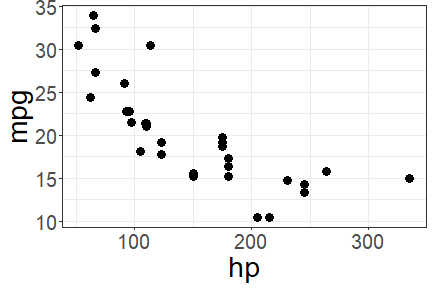
\includegraphics[width=0.55\linewidth]{ESM_week4_nls_pres_files/figure-beamer/mtcars-1} \end{center}

How does OLS fit the line?

\begin{itemize}[<+->]
\tightlist
\item
  Hint:
  \(\hat{\beta}=\frac{\sum^n_{i=1}(x_i-\bar{x})(y_i-\bar{y})}{\sum^n_{i=1}(x_i-\bar{x})^2}\)
\end{itemize}
\end{frame}

\begin{frame}{Remember what OLS does first}
\protect\hypertarget{remember-what-ols-does-first-1}{}
How does OLS fit the line?

\begin{itemize}
\tightlist
\item
  Minimize squared error (aka residuals)
\end{itemize}

\[
\hat\beta=\min_\beta \sum^n_{i=1}\hat{\epsilon_i}^2=\sum^n_{i=1}(y_i-\beta x_i)^2
\]

\begin{center}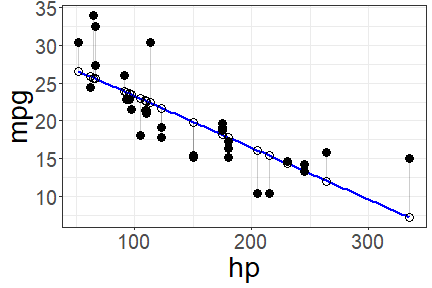
\includegraphics[width=0.55\linewidth]{ESM_week4_nls_pres_files/figure-beamer/unnamed-chunk-1-1} \end{center}
\end{frame}

\begin{frame}{OLS is simple and powerful, but has limitations}
\protect\hypertarget{ols-is-simple-and-powerful-but-has-limitations}{}
\begin{itemize}
\item
  Linear relationship between predictor (y) and variables (x)
\item
  Last week we started branching away from linear models with logistic
  regressions
\item
  But the link functions typically still maintain a linear form
\end{itemize}

\[
\ln(\frac{p}{1-p})=\beta_0+\beta_1x_1+\beta_2x_2+...\beta_nx_n
\]
\end{frame}

\begin{frame}{But what if we get something like this?}
\protect\hypertarget{but-what-if-we-get-something-like-this}{}
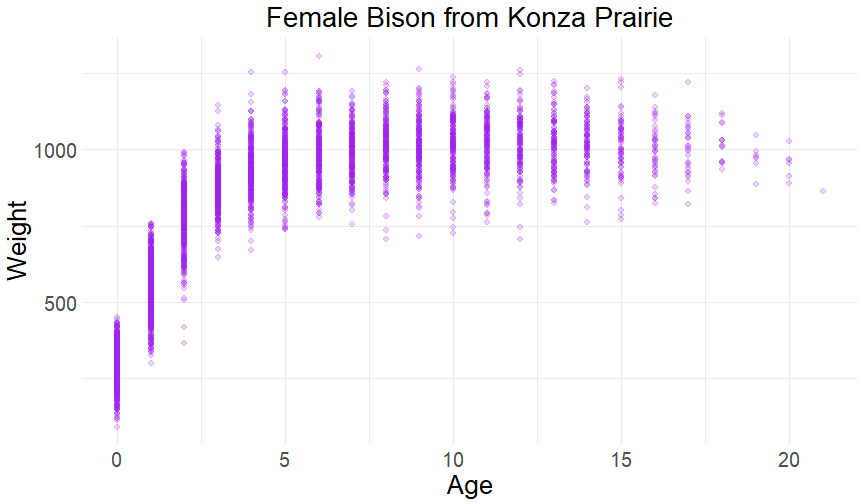
\includegraphics{ESM_week4_nls_pres_files/figure-beamer/unnamed-chunk-2-1.pdf}
\end{frame}

\begin{frame}{Or this?}
\protect\hypertarget{or-this}{}
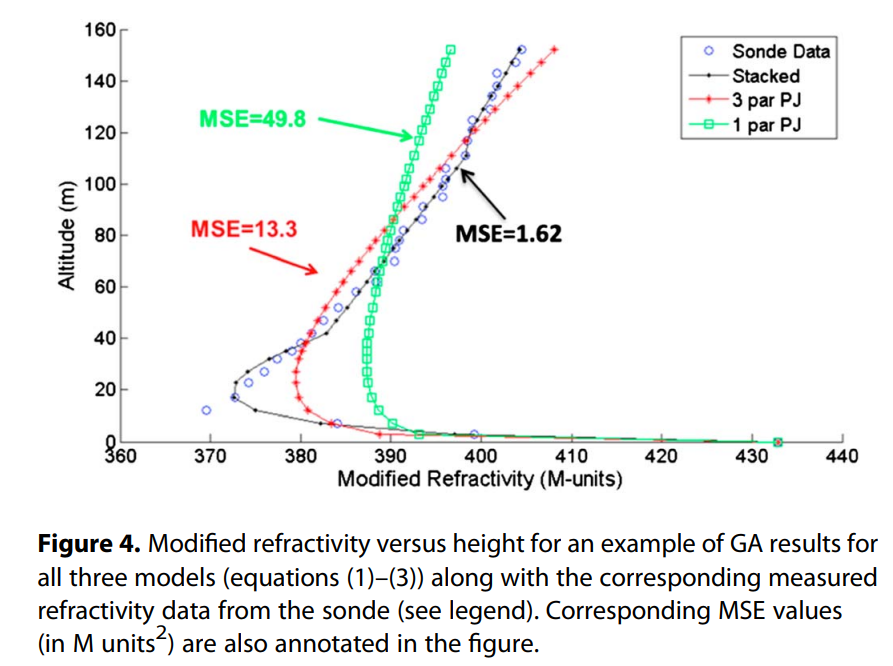
\includegraphics{refractivity.PNG}
\end{frame}

\begin{frame}{In specific applications, accuracy greatly matters!}
\protect\hypertarget{in-specific-applications-accuracy-greatly-matters}{}
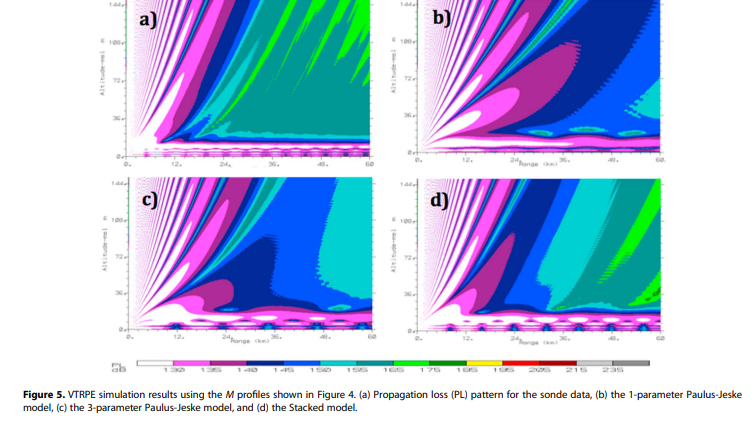
\includegraphics{vtrpe_run.PNG}
\end{frame}

\begin{frame}{Nonlinear Least Squares}
\protect\hypertarget{nonlinear-least-squares}{}
Apply the same idea of least squares error minimization, but with any
function

\begin{equation}
y_i=f(x_i,\boldsymbol\beta)+\epsilon_i 
\end{equation}

\begin{equation}
\min_{\boldsymbol\beta}=\sum^n_{i=1}\epsilon_i^2=\sum^n_{i=1}(y_i-f(x_i,\boldsymbol\beta))^2
\end{equation}

General idea is very similar, but implementation and use is quite
different
\end{frame}

\begin{frame}{How NLS works}
\protect\hypertarget{how-nls-works}{}
No simple analytical solution like in OLS (Solve for \(\hat\beta\))

Instead we iteratively approximate the solution through algorithms

\begin{itemize}
\item
  Gauss-Newton (Most Common)
\item
  Levenberg-Marquardt (More flexible)
\end{itemize}

In general the algorithms make an approximation of the functions
gradient (think derivative), then move along until some convergence
criteria is met

\[
|\frac{\overbrace{S^k}^{\text{Previous squared errror}}-\overbrace{S^{k+1}}^{\text{Updated squared error}}}{S^k}|<0.0001
\]
\end{frame}

\begin{frame}
\href{https://www1.hft-leipzig.de/strutz/Animations/op.html}{Demonstration
of Gauss Newton Algorithm}

When viewing the Gifs at the link, see how important the initial
position of the guess is to avoid being trapped.

\footnotesize

(A weakness in Beamer is not being able to include gifs, it is a pdf
afterall!)
\end{frame}

\begin{frame}{Why should we use NLS?}
\protect\hypertarget{why-should-we-use-nls}{}
We need far fewer assumptions than even multiple regression

\begin{itemize}
\item
  Residuals do not have to be normally distributed
\item
  No linear relationship required
\item
  Don't care about homoscedasticity
\end{itemize}

If underlying model is smooth, can find solutions accurately and quickly
compared to other methods
\end{frame}

\begin{frame}{When to use NLS}
\protect\hypertarget{when-to-use-nls}{}
Best suited for specific model parameterization given a collection of
data

NLS excels when we have a known equation and want to fit parameters

There is no \(R^2\) value to compare across model specifications, but we
can still test model performance using AIC or Cross Fold Validation
through RMSE (In lab this week!)

NLS is particularly useful for time series, but we will cover other
methods for time series later in class.
\end{frame}

\begin{frame}{Pitfalls (literally) and warnings}
\protect\hypertarget{pitfalls-literally-and-warnings}{}
\begin{cols}

\begin{col}{0.475\textwidth}

NLS is only as good as the underlying model. Bring your brain to the
party and make sure the model you're fitting is appropriate

Follows gradient of steepest descent \(\rightarrow\) local min/max
valleys

\begin{itemize}
\tightlist
\item
  With n-parameters chances of local min/max rises
\end{itemize}

\end{col}

\begin{col}{0.05\textwidth}

~

\end{col}

\begin{col}{0.475\textwidth}

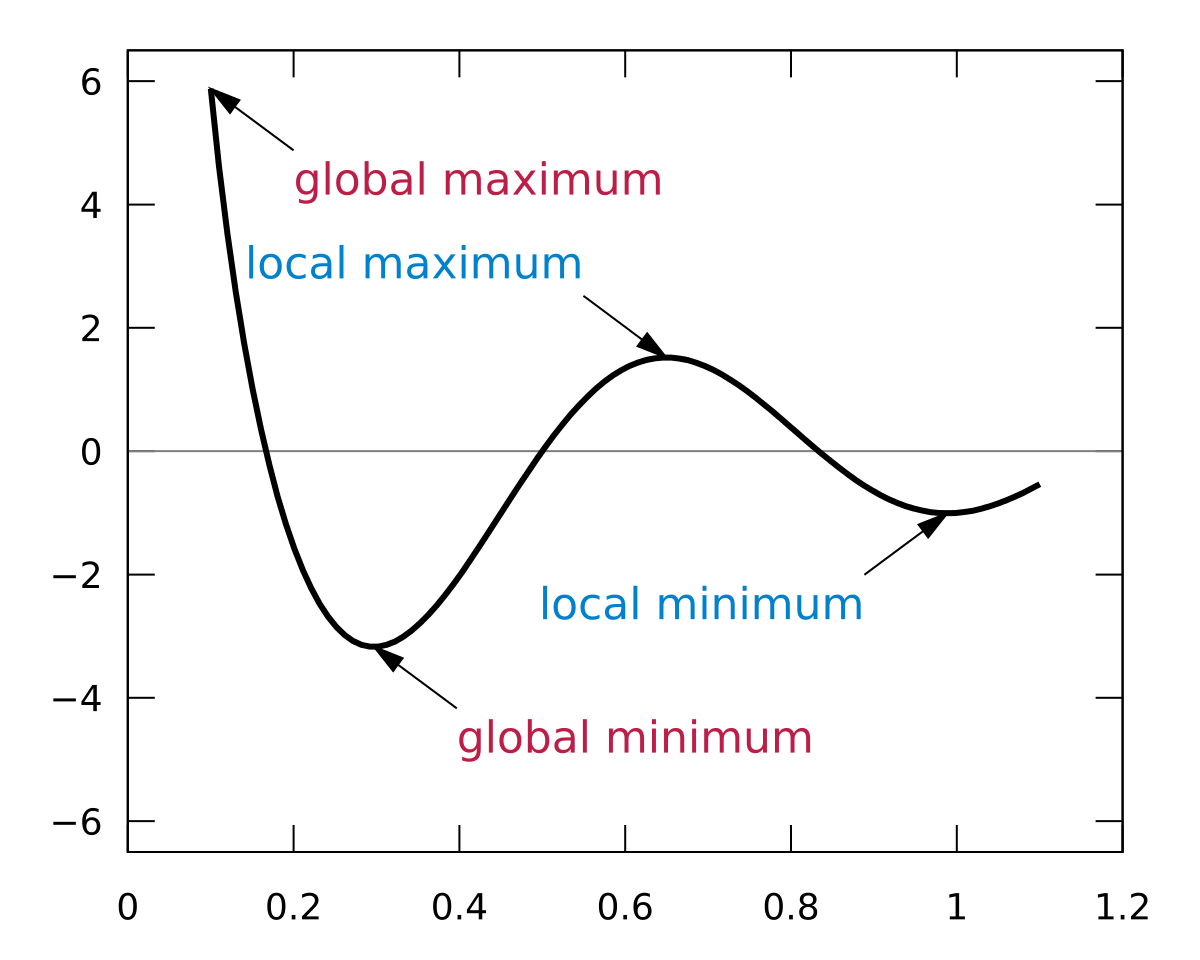
\includegraphics{minmax.png}

Requires good initial guesses

\begin{itemize}
\tightlist
\item
  Comes from the underpinning algorithms
\end{itemize}

\end{col}

\end{cols}
\end{frame}

\begin{frame}{Know when to use NLS or another option}
\protect\hypertarget{know-when-to-use-nls-or-another-option}{}
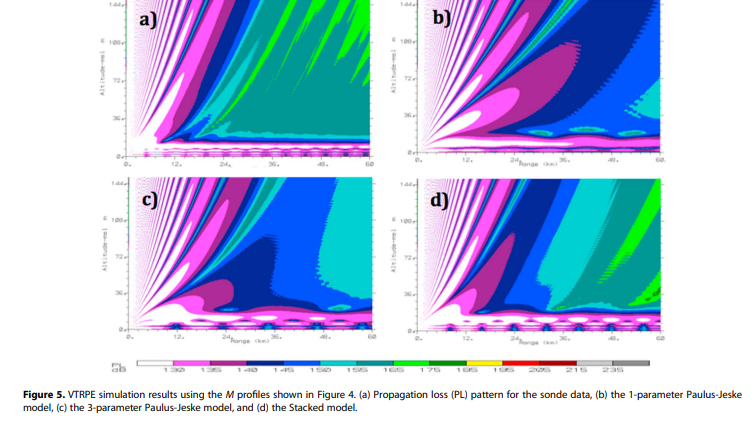
\includegraphics{vtrpe_run.PNG}

In this research we ended up using Genetic Algorithms instead as they
provide global solutions without having to guess

Operationally, the Navy doesn't have time to guess
\end{frame}

\hypertarget{using-nls-in-r}{%
\section{Using NLS in R}\label{using-nls-in-r}}

\begin{frame}[fragile]{Let's apply NLS to our Female Bisons}
\protect\hypertarget{lets-apply-nls-to-our-female-bisons}{}
\begin{Shaded}
\begin{Highlighting}[]
\NormalTok{knz\_bison\_age }\OtherTok{\textless{}{-}}\NormalTok{ knz\_bison }\SpecialCharTok{\%\textgreater{}\%} 
  \FunctionTok{mutate}\NormalTok{(}\AttributeTok{animal\_age =}\NormalTok{ rec\_year }\SpecialCharTok{{-}}\NormalTok{ animal\_yob) }\SpecialCharTok{\%\textgreater{}\%} 
  \FunctionTok{filter}\NormalTok{(animal\_sex}\SpecialCharTok{==}\StringTok{"F"}\NormalTok{)}
\end{Highlighting}
\end{Shaded}

\begin{center}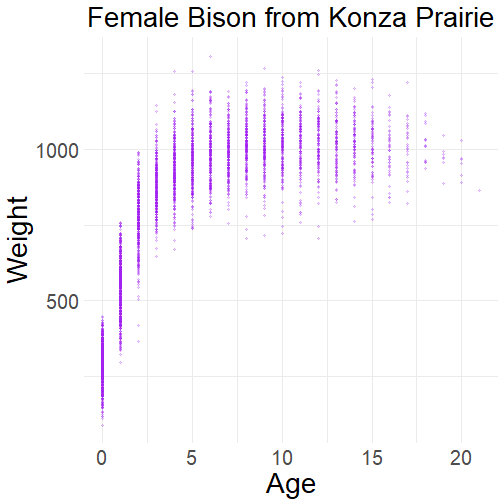
\includegraphics[height=0.75\textheight]{ESM_week4_nls_pres_files/figure-beamer/bisongraph-1} \end{center}
\end{frame}

\begin{frame}[fragile]{Use R Built in functions}
\protect\hypertarget{use-r-built-in-functions}{}
\begin{Shaded}
\begin{Highlighting}[]
\NormalTok{df\_nls}\OtherTok{\textless{}{-}}\FunctionTok{nls}\NormalTok{(}\AttributeTok{formula=}   \CommentTok{\# Model we want to estimate,}
\NormalTok{            data   }\CommentTok{\# Data we are evaluating,}
\NormalTok{            start  }\CommentTok{\# Our initial guesses}
\NormalTok{            control }\CommentTok{\# List of tolerance value, etc}
\NormalTok{            trace  }\CommentTok{\# Do we want to see convergence}
\NormalTok{            upper  }\CommentTok{\# Bounds on input parameters}
\NormalTok{            ... }\CommentTok{\# some other useful stuff )}
\end{Highlighting}
\end{Shaded}
\end{frame}

\begin{frame}{What Model to use?}
\protect\hypertarget{what-model-to-use}{}
Scour the literature or create your own (only with sufficient
justification)

For our Bison, Martin and Barboza (2020) used a Gompertz model

\begin{equation}
BM=b1*exp(-exp(-b2*(age-b3)))
\end{equation}

\begin{cols}

\begin{col}{0.475\textwidth}

\tiny

\(b1\) = asymptotic body mass (pounds)

\(b2\) = instantaneous growth-rate

\(b3\) = age at inflection point years

\(age\) = Independent variable

\(BM\) = Body mass (pounds) Dependent variable

\end{col}

\begin{col}{0.05\textwidth}

~

\end{col}

\begin{col}{0.475\textwidth}

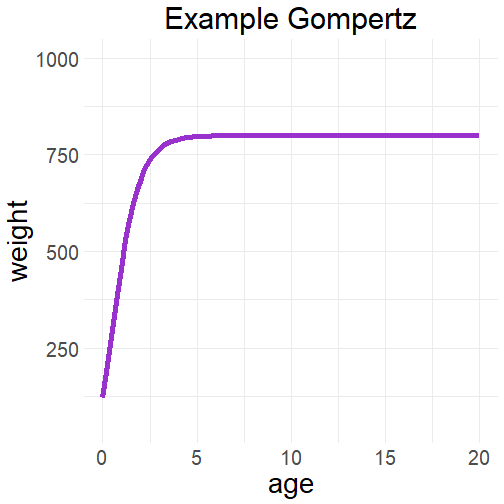
\includegraphics[width=0.9\linewidth]{ESM_week4_nls_pres_files/figure-beamer/gompertz-1}

\end{col}

\end{cols}
\end{frame}

\begin{frame}[fragile]{Create a function in R to test our model}
\protect\hypertarget{create-a-function-in-r-to-test-our-model}{}
\begin{Shaded}
\begin{Highlighting}[]
\NormalTok{gompertz}\OtherTok{\textless{}{-}}\ControlFlowTok{function}\NormalTok{(b1,b2,b3,age)\{}
\NormalTok{ BM}\OtherTok{=}\NormalTok{ b1}\SpecialCharTok{*}\FunctionTok{exp}\NormalTok{(}\SpecialCharTok{{-}}\FunctionTok{exp}\NormalTok{(}\SpecialCharTok{{-}}\NormalTok{b2}\SpecialCharTok{*}\NormalTok{(age}\SpecialCharTok{{-}}\NormalTok{b3)))}
\FunctionTok{return}\NormalTok{(BM)}
\NormalTok{\}}
\end{Highlighting}
\end{Shaded}

\small

Note: For the nls function it's okay to define all parameters like we
did. In other optimization tools (e.g.~optim) you would want to keep the
first input index as a vector if you have multiple choice variables
\end{frame}

\begin{frame}[fragile]{Providing a guess is very important}
\protect\hypertarget{providing-a-guess-is-very-important}{}
\begin{Shaded}
\begin{Highlighting}[]
\NormalTok{df\_nls}\OtherTok{\textless{}{-}}\FunctionTok{nls}\NormalTok{(animal\_weight}\SpecialCharTok{\textasciitilde{}}\FunctionTok{gompertz}\NormalTok{(b1,b2,b3,animal\_age),   }
            \AttributeTok{data=}\NormalTok{knz\_bison\_age,   }
            \AttributeTok{start=}\FunctionTok{list}\NormalTok{(}\AttributeTok{b1=}\NormalTok{?,}\AttributeTok{b2=}\NormalTok{?,}\AttributeTok{b3=}\NormalTok{?),}
            \AttributeTok{trace=}\ConstantTok{TRUE}\NormalTok{ )}
\end{Highlighting}
\end{Shaded}

The initial guesses and data also tell nls which variables are we trying
to find and which data are we comparing
\end{frame}

\begin{frame}{4 methods for providing guesses}
\protect\hypertarget{methods-for-providing-guesses}{}
\begin{enumerate}
[1)]
\item
  Use past parameters from similar studies
\item
  Use data to internally define guesses (min, mean, max, etc.)
\item
  In 2-D, look at the graphs and estimate
\item
  In N-D, combine steps 1-2 then create a start grid to search over
\end{enumerate}
\end{frame}

\begin{frame}{Applied guessing}
\protect\hypertarget{applied-guessing}{}
\small

How we could use step 2 and 3 in this case

Asymptotic body mass (\(b1\)) implies a max body length we could take
the biggest observed female or generally look at the graph

Age inflection point (\(b3\)) is where the curve starts bending

Instantaneous growth-rate (\(b2\)) is kind of weird, but you could
manipulate a set Gompertz model to see how it changes the shape and try
to match it.

\begin{center}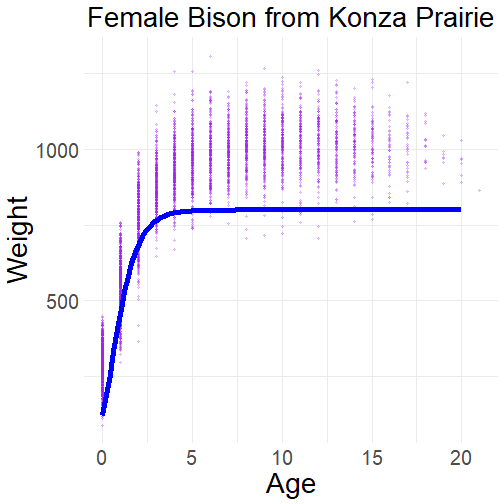
\includegraphics[height=0.5\textheight]{ESM_week4_nls_pres_files/figure-beamer/combeinplot-1} \end{center}
\end{frame}

\begin{frame}[fragile]{Apply guesses}
\protect\hypertarget{apply-guesses}{}
\small

\begin{Shaded}
\begin{Highlighting}[]
\NormalTok{b\_gompertz}\OtherTok{\textless{}{-}}\FunctionTok{nls}\NormalTok{(animal\_weight}\SpecialCharTok{\textasciitilde{}}\FunctionTok{gompertz}\NormalTok{(b1,b2,b3,animal\_age),}
                      \AttributeTok{data =}\NormalTok{ knz\_bison\_age,}
                      \AttributeTok{start =} \FunctionTok{list}\NormalTok{(}\AttributeTok{b1=}\DecValTok{1000}\NormalTok{,}\AttributeTok{b2=}\DecValTok{1}\NormalTok{,}\AttributeTok{b3=}\FloatTok{0.6}\NormalTok{),}
                      \AttributeTok{trace =} \ConstantTok{TRUE}\NormalTok{)}
\end{Highlighting}
\end{Shaded}

\begin{verbatim}
## 52917148 :  1e+03 1e+00 6e-01
## 34426629 :  1007.2008456    0.6930941    0.3444975
## 33207967 :  1009.6701568    0.7250854    0.2798164
## 33206308 :  1009.7635726    0.7275290    0.2832794
## 33206307 :  1009.7560207    0.7275973    0.2832921
\end{verbatim}
\end{frame}

\begin{frame}[fragile]{What did the model find?}
\protect\hypertarget{what-did-the-model-find}{}
\footnotesize

\begin{Shaded}
\begin{Highlighting}[]
\FunctionTok{summary}\NormalTok{(b\_gompertz)}
\end{Highlighting}
\end{Shaded}

\begin{verbatim}
## 
## Formula: animal_weight ~ gompertz(b1, b2, b3, animal_age)
## 
## Parameters:
##     Estimate Std. Error t value Pr(>|t|)    
## b1 1.010e+03  1.903e+00  530.58   <2e-16 ***
## b2 7.276e-01  7.550e-03   96.38   <2e-16 ***
## b3 2.833e-01  8.064e-03   35.13   <2e-16 ***
## ---
## Signif. codes:  0 '***' 0.001 '**' 0.01 '*' 0.05 '.' 0.1 ' ' 1
## 
## Residual standard error: 81.12 on 5046 degrees of freedom
## 
## Number of iterations to convergence: 4 
## Achieved convergence tolerance: 3.106e-06
##   (236 observations deleted due to missingness)
\end{verbatim}
\end{frame}

\begin{frame}{How well does the model predict the data?}
\protect\hypertarget{how-well-does-the-model-predict-the-data}{}
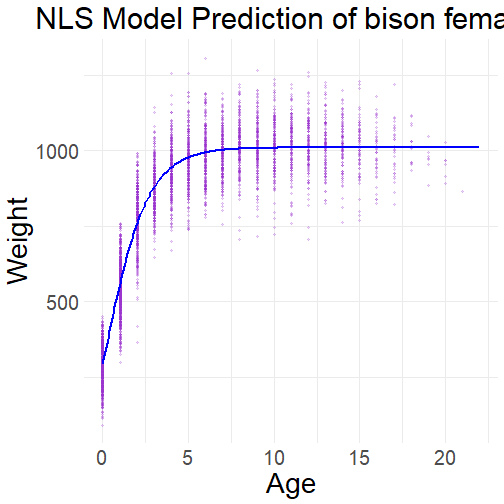
\includegraphics{ESM_week4_nls_pres_files/figure-beamer/unnamed-chunk-3-1.pdf}
\end{frame}

\begin{frame}[fragile]{}
\protect\hypertarget{section}{}
\begin{Shaded}
\begin{Highlighting}[]
\NormalTok{model\_aug}\OtherTok{\textless{}{-}}\NormalTok{broom}\SpecialCharTok{::}\FunctionTok{augment}\NormalTok{(b\_gompertz)}

\NormalTok{sum\_squared\_error}\OtherTok{=}\FunctionTok{sum}\NormalTok{((model\_aug}\SpecialCharTok{$}\NormalTok{.resid)}\SpecialCharTok{\^{}}\DecValTok{2}\NormalTok{)}
\FunctionTok{print}\NormalTok{(sum\_squared\_error)}
\end{Highlighting}
\end{Shaded}

\begin{verbatim}
## [1] 33206307
\end{verbatim}

If we compare different model runs from the trace output we can see this
is the smallest sum of squared errors. No other model will get lower
this number.
\end{frame}

\begin{frame}[fragile]{Adding confidence intervals is easy}
\protect\hypertarget{adding-confidence-intervals-is-easy}{}
\small

\begin{Shaded}
\begin{Highlighting}[]
\NormalTok{conf}\OtherTok{\textless{}{-}}\FunctionTok{as\_tibble}\NormalTok{(}\FunctionTok{predFit}\NormalTok{(b\_gompertz,}
            \AttributeTok{newdata =} \FunctionTok{list}\NormalTok{(}\AttributeTok{animal\_age=}\NormalTok{age\_series),}
            \AttributeTok{interval=}\StringTok{"confidence"}\NormalTok{),}
            \AttributeTok{level=}\FloatTok{0.95}\NormalTok{) }

\FunctionTok{head}\NormalTok{(conf,}\AttributeTok{n=}\DecValTok{4}\NormalTok{)}
\end{Highlighting}
\end{Shaded}

\begin{verbatim}
## # A tibble: 4 x 3
##     fit   lwr   upr
##   <dbl> <dbl> <dbl>
## 1  295.  291.  300.
## 2  322.  318.  327.
## 3  349.  345.  353.
## 4  376.  372.  380.
\end{verbatim}

\begin{Shaded}
\begin{Highlighting}[]
\CommentTok{\#plot+geom\_ribbon(data=conf...)}
\end{Highlighting}
\end{Shaded}

Model fits so well, the confidence intervals don't even show on plot.
\end{frame}

\hypertarget{optimization-across-r}{%
\section{Optimization across R}\label{optimization-across-r}}

\begin{frame}{NLS falls under the optimization umbrella}
\protect\hypertarget{nls-falls-under-the-optimization-umbrella}{}
Many flavors and varieties of optimization

As simply as possible

\[
\begin{aligned}
V(x,c)&=\max_cf(x,c) &\text{Subject to}\\
x&\ge0 \\
c&\ge 0  \\
x&=g(x,c)
\end{aligned}
\]
\end{frame}

\begin{frame}{Which method to use?}
\protect\hypertarget{which-method-to-use}{}
Depends on the question being asked

\begin{itemize}
\item
  What mathematical form is the optimization equation in?

  \begin{itemize}
  \tightlist
  \item
    Something like Maximum likelihood estimatation will be different
    than quadratic programming
  \end{itemize}
\item
  Do I need it to be fast or accurate?
\item
  How many/form of parameters?
\end{itemize}

Best to use methods that you understand than ones you don't
\end{frame}

\begin{frame}{Optimization toolkit highlights}
\protect\hypertarget{optimization-toolkit-highlights}{}
\small

optim/optimx: Workhorse functions in R and probably the ones you will
use the most

-\href{https://www.jstatsoft.org/article/download/v060i02/788}{Article
on why we should move towards optimx}

quadprog: \href{https://www.fishwallet.net/}{Used by a GP I advised in
2021}

GA: Genetic algorithms are the best global tool that I know of

NLoptr:
\href{https://nlopt.readthedocs.io/en/latest/NLopt_Introduction/}{New
project trying to keep syntax of alogrithms the same across computer
languages}

\href{https://cran.r-project.org/web/views/Optimization.html}{List of
every optimization function with short descriptions}
\end{frame}

\end{document}
